
\section{Visualizing language-specific distributions}\label{sec:LanguageSpecific}

Even in a contrastive study, the first step consists in the inspection
of the language-specific distributions. We mostly deal with four such
distributions if we study two languages $L_1$ and $L_2$: 
$L_1$/original, $L_1$/translated (from $L_2$), $L_2$/original, and
$L_2$/translated (from $L_1$). By inspecting these distributions we
can gain a first impression of the differences between $L_1$ and
$L_2$, as well as between the original and translated
versions of both languages.

In this section we discuss three types of visualization techniques,
summarized under `proportional geometric visualizations'
(Sect. \ref{sec:PropGeom}), `graph-based visualizations'
(Sect. \ref{sec:CCCG}), and `ordination techniques'
(Sect. \ref{sec:Ordination}).

\subsection{Proportional geometric visualizations}\label{sec:PropGeom}

Among the techniques most commonly used for the visualization of
monolingual data are what we can loosely call `proportional plots',
where frequencies observed in data are graphically represented in such
a way that the size of some geometric shape is 
proportional to them. The most widely used plot types are
probably mosaic plots and Cohen-Friendly association plots
(\citealt{Cohen1980,Friendly1992,Friendly1994}). We will focus on mosaic plots,
using the \verb+vcd+ package for \verb+R+.\footnote{Mosaic plots can
  also be generated with the Python module \verb+statsmodels+.}
Consider Figure \ref{fig:mosaicplots1-2}. The contingency table at the
top shows how frequently the French \pradv s
\textit{immédiatement}, \textit{tout de suite} and \textit{bientôt}
are used with chronological or deictic reference points (i.e., with
reference points in the surrounding text, as in (\ref{ex1}), or with
the moment of speech as the reference point, as in (\ref{ex2})).
%
Each cell in the table corresponds to a combination of levels from the two
variables \textsc{\pradv} and \textsc{Reference Point}.
%
The rectangles in the mosaic plot at the bottom are proportional in size to
the frequencies shown in the table at the top along both
dimensions. Along the $x$-axis their length corresponds to the
proportion of the relevant level within the category \textsc{French
  \pradv}, and along the $y$-axis the rectangles reflect the
proportion of deictic and chronological observations.
%
The mosaic plot shows, among other things, that the cells
corresponding to chronological/\textit{immédiatement} (top left) and
deictic/\textit{immédiatement} (bottom left), while exhibiting rather
similar counts (32 and 29), exhibit very different relative
frequencies in the rows for chronological and deictic cases.

\begin{figure}[t]
  \centering
  {\footnotesize
    \begin{tabular}[h]{llll}
                   &    \rot{immédiatement} & \rot{tout de suite} &  \rot{bientôt}\\
  chronological    &        32        &    15         &   3     \\ 
  deictic          &        29        &    41         &   97    \\
    \end{tabular}
  } 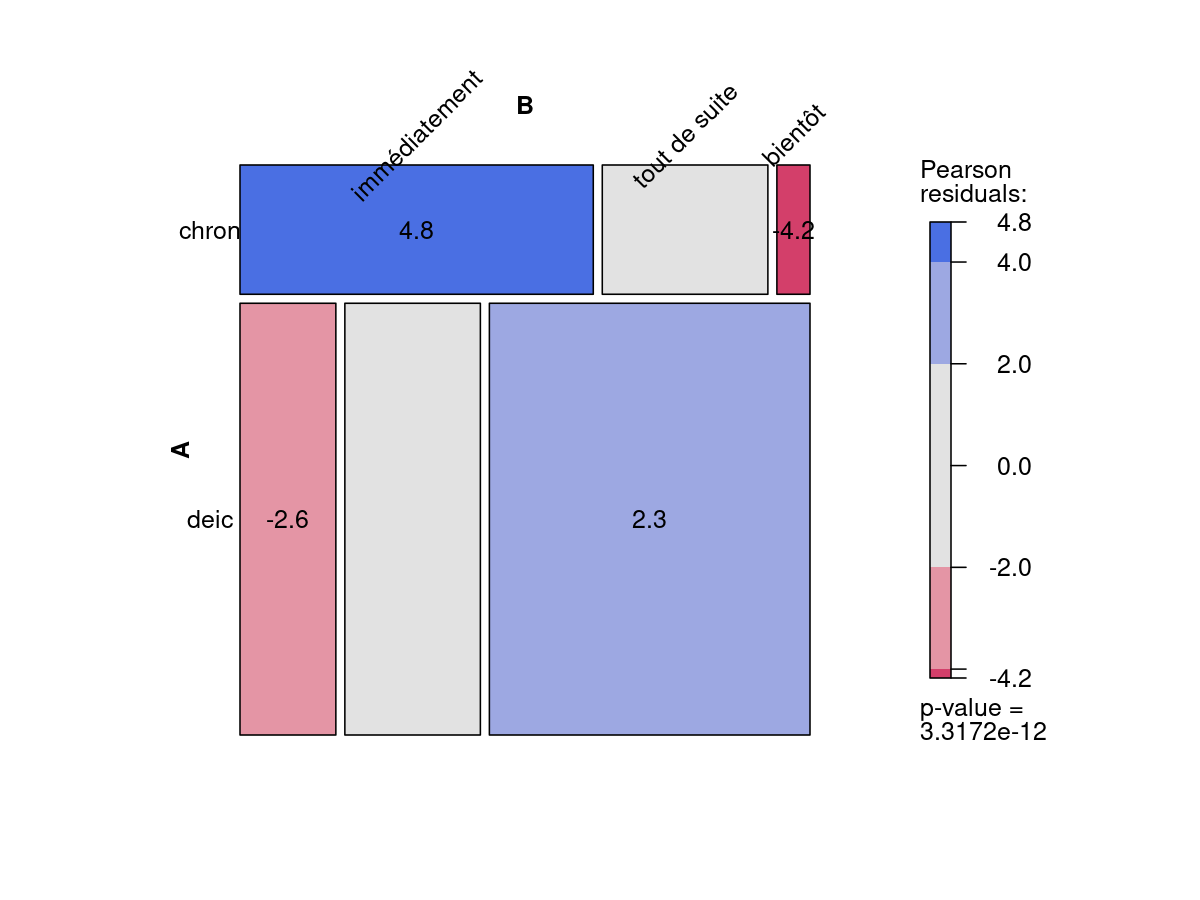
\includegraphics[width=0.9\linewidth]{figures/mosaic-fr-ref-ip.png}
  \cprotect\caption{Contingency table (top) and mosaic plot (bottom)
    representing the frequencies as well as degrees of over- or
    underrepresentation for three French \pradv-adverbials relative to
    the variable \textsc{reference point} (\textit{chron}:
    chronological, \textit{deic}: deictic). The plot was created with
    the package \verb+vcd+ for \verb+R+ (\citealt{vcd-package});
    cf. the script \verb+01_proportional_visualizations.R+ in the
    Supplementary Materials.}
  \label{fig:mosaicplots1-2}
\end{figure}
%
Figure \ref{fig:mosaicplots1-2} also provides information about levels
of deviation from statistical independence (a homogeneous distribution). The
colour of a rectangle corresponding to a cell $C_{m,n}$ of a
contingency table $C$ reflects the magnitude of the Pearson residuals
$E_{m,n}$ for $C_{m,n}$ (cf. \citealt[Ch. 3]{Agresti2002} for
details). Pearson residuals can be regarded as a standardized measure
of deviation from statistical independence. They are calculated as the
difference between the observed and expected frequency, divided by the
square root of the expected frequency (see
Sect. \ref{sec:PearsonResds} in the Appendix for some
explanations). Pearson residuals approximately follow a standard
normal distribution (but see below for a caveat), which means that we
can estimate the probability of a cell count, given the assumption of
statistical independence (homogeneity): $\approx 68\%$ of the data are
located within one standard deviation of the distribution, and
$\approx 95\%$ are located within two standard distributions. As we
are typically interested in results beyond the 95\% threshold
($\alpha=0.05$, for an undirected hypothesis), the thresholds $2$
(for overrepresentation) and $-2$ for underrepresentation are
particularly relevant.

As the legend to the right of the plot shows, the colours indicate the
following magnitudes: light blue: $4 > E_{m,n} > 2$, dark blue: $E_{m,n}>4$,
light red: $-4 < E_{m,n} < -2$, dark red: $E_{m,n}<-4$. In cells with a
significant over- or underrepresentation the Pearson residuals are
moreover specified in the relevant rectangle.
The plot suggests that \textit{immédiatement} tends to co-occur
with chronological reference points, while \textit{bientôt} is
attracted by deictic reference points. \textit{Tout de suite} does not
seem to show a particular association with either type of reference
point.

An important point to note is that Pearson residuals do not exactly
follow a standard normal distribution and ``[provide] conservative
indications of cells having lack of fit'' \citep[81]{Agresti2002}.
Alternatively, an ``adjusted'' residual, which ``results from dividing
it by its standard error'', can be used (\citealt[81]{Agresti2002}). In
the context of mosaic plots, \citet[7]{Friendly1994b} notes that ``the
adjusted residuals are always larger in magnitude than the unadjusted
values'', and ``adjusted residuals have the property that their
standard errors are equal, so their values are more comparable over
cells in the contingency table''. He also holds that ``experience
shows that they provide \textit{better visual display of the patterns
  of association} than do ordinary Pearson \ldots %or LR [linear regression]
residuals'' (emphasis original).

\begin{figure}[t]
  \centering
  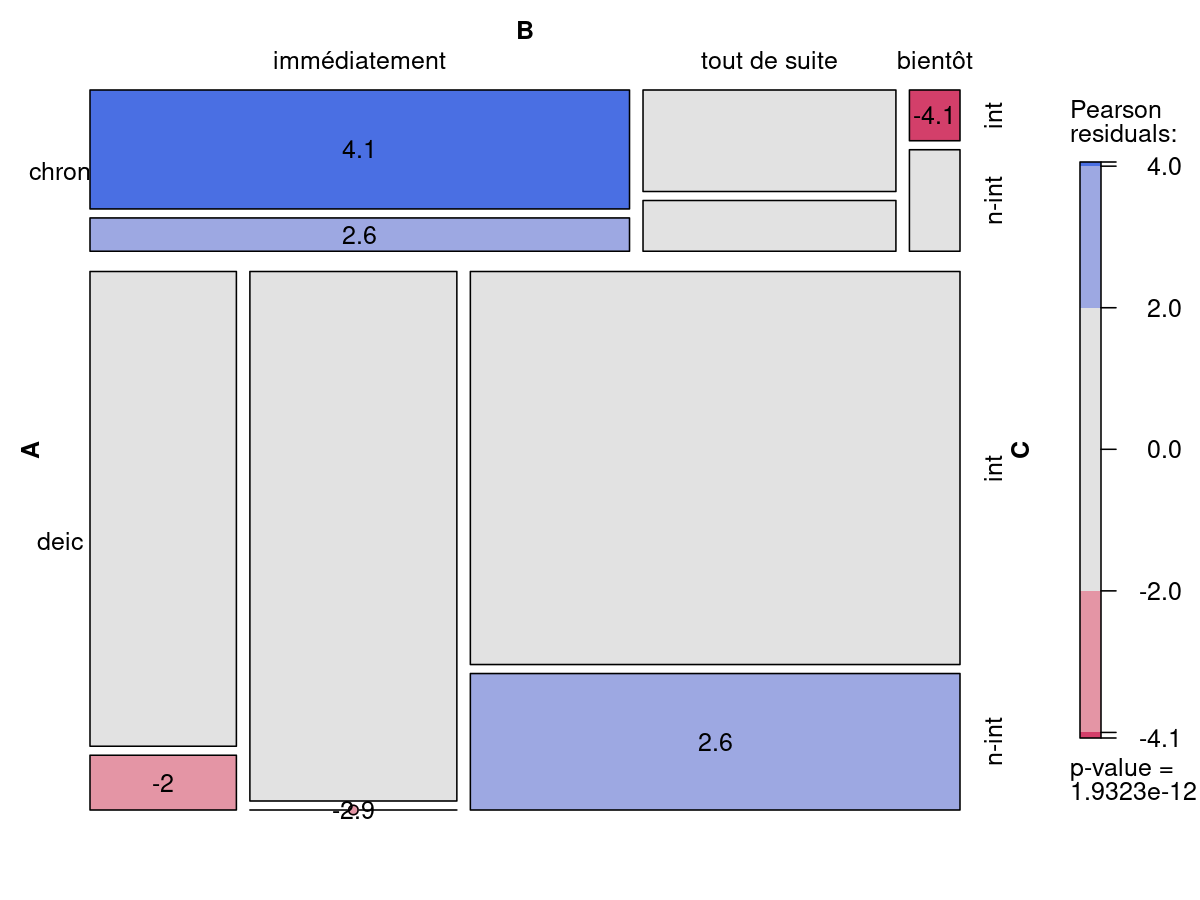
\includegraphics[width=0.9\linewidth]{figures/mosaic-fr-ref-ip-int.png}
  \cprotect\caption{Mosaic plot representing the frequencies as well
    as degrees of over- or underrepresentation for three French
    \pradv-adverbials relative to the variables \textsc{reference
      point} (\textit{chron}: chronological, \textit{deic}: deictic)
    and \textsc{Intentionality} (\textit{int}: intentional,
    \textit{n-int}: non-intentional). The plot was created with the
    package \verb+vcd+ for \verb+R+ (\citealt{vcd-package}); cf. the
    script \verb+01_proportional_visualizations.R+ in the
    Supplementary Materials.}
  \label{fig:2D}
\end{figure}


As we do not focus on inferential statistics in this contribution, we
will not go into any further details at this point (but see
Sect. \ref{sec:PearsonResds} in the Appendix for some
comments). Readers and users should be aware of the ``meaning'' of the
colours in a mosaic plot, however, and take it into account in their
interpretation of the data.
In the following, we will continue to use unadjusted Pearson residuals for the
sake of simplicity, because they also play an important role in
ordination (where they are mostly called `standardized
residuals', see Sect. \ref{sec:Ordination}).

So far we have only crossed two variables. Figure \ref{fig:2D} shows a
mosaic plot where three variables have been crossed: (French)
\textsc{\pradv}, \textsc{Reference Point} and
\textsc{Intentionality}. In this case the (graphically) two-dimensional
representation provided by a mosaic plot has its limitations, and the
diagram effectively shows two plots, one at the top, where
\textsc{Intentionality} is crossed with \textsc{\pradv} for
chronological reference points, and one at the bottom, where this
combination is shown for deictic reference
points. % The information about the residuals
% represented by the colours is based on numbers from the entire
% distribution though.
We can see that three combinations have Pearson residuals higher than $2$:
\{chronological, intentional, \textit{immédiatement}\},
\{chronological, non-intentional, \textit{immédiatement}\},
and \{deictic, non-intentional, \textit{bientôt}\}. \{Deictic,
non-intentional, \textit{immédiatement}\} and \{deictic,
non-intentional, \textit{tout de suite}\} and \{chronological,
intentional, \textit{bientôt}\} have residuals lower than $-2$.

An alternative way of visualizing three-dimensional distributions is
shown in Figure \ref{fig:3D}, in what we call a Feature-Combination
Frequency Grid (FCFG) (see \citealt{Gast2017Even}).  Each node in the
grid corresponds to one feature combination, and the size of a sphere
represents the observed or expected frequency of the relevant feature
combination. The colours of the spheres reflect Pearson
residuals, as in mosaic plots.

\begin{figure}[t]
  \centering
  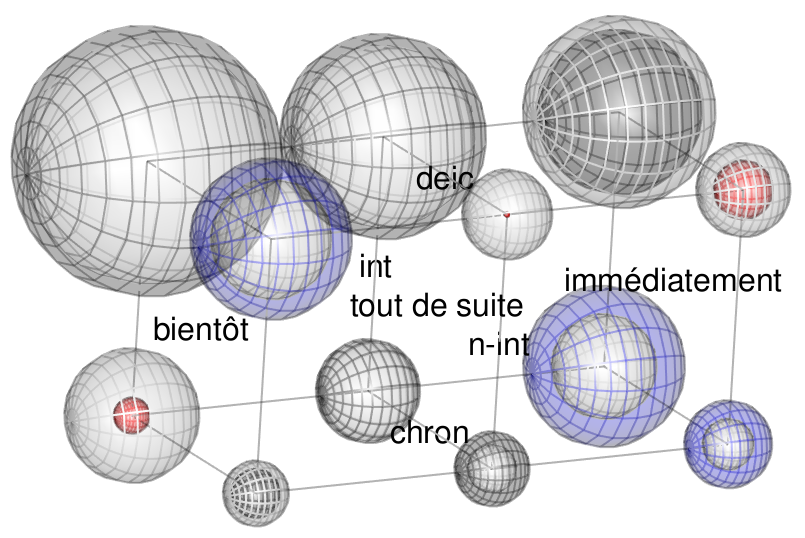
\includegraphics[width=0.5\linewidth]{figures/FCF-grid-ImPost.png}
  \cprotect\caption{Feature-Combination Frequency Grid (FCFG)
    representing the frequencies as well as degrees of over-
    or underrepresentation for three French \pradv s relative
    to the variables \textsc{Illocutionary force} and
    \textsc{Intentionality} (see Fig. \ref{fig:2D} for the
    levels). The visualization was created using the package
    \verb+rgl+ for R; cf. the script
    \verb+01_proportional_visualizations.R+.}
  \label{fig:3D}
\end{figure}


\subsection{Context-Conditional Correlation Graphs}\label{sec:CCCG}

With Feature-Combination Frequency Grids (FCFGs) we can maximally
visualize data along three dimensions. More dimensions are possible
with `stacked' mosaic plots as shown in Figure
\ref{fig:2D}, but the information becomes increasingly difficult
to process as the number of dimensions increases. In order to represent
pairwise associations of variables in a single plot we can make use of
graphs. We call graphs of the type shown in Figure \ref{fig:CCCG}
Context-Conditional Correlation Graphs (CCCG). The graph illustrates
(significant) imbalances in the distribution of German \pradv s
relative to four variables (\textsc{Intentionality}, \textsc{Agent},
\textsc{Reference point} and \textsc{Illocutionary
  force/Modality}).\footnote{Variables and levels:
  \textsc{Agent}: \textit{Ag$x$Ps}
  indicates that \textsc{Agent} is $x$. person;
  %
  \textsc{Illocutionary force/modality}: 
  \textit{dir.boul}: directive/bouletic,
  \textit{n.illoc}: not indicated,
  \textit{poss}: possibility;
  %
  \textsc{Intentionality}: \textit{int}: intentional predicate,
  \textit{n.int}: non-intentional predicate; \textsc{Reference point}:
  \textit{chron}: chronological, \textit{deic}: deictic;
  \textsc{Modification}: \textit{modf}: adverbial is syntactically
  modified, \textit{n-modf}: adverbial is not syntactically
  modified.\label{FigNote1}} The arcs show, for each pair of variables,
the levels for which there is a significant overrepresentation in a
pairwise cross-tabulation, along with the Pearson residual (following
the underscore). For example, the arc at the very top shows that in a
cross-table $T$ of the variables \textsc{\pradv} and \textsc{Agent},
the Pearson residual for the cell $T_{3rd,bald}\approx 4$. The
location of `Ag3ps\_4' (closer to \textit{bald} than to
\textit{gleich}) indicates that this feature is overrepresented for
\textit{bald}.

\begin{figure}[t]
  \centering 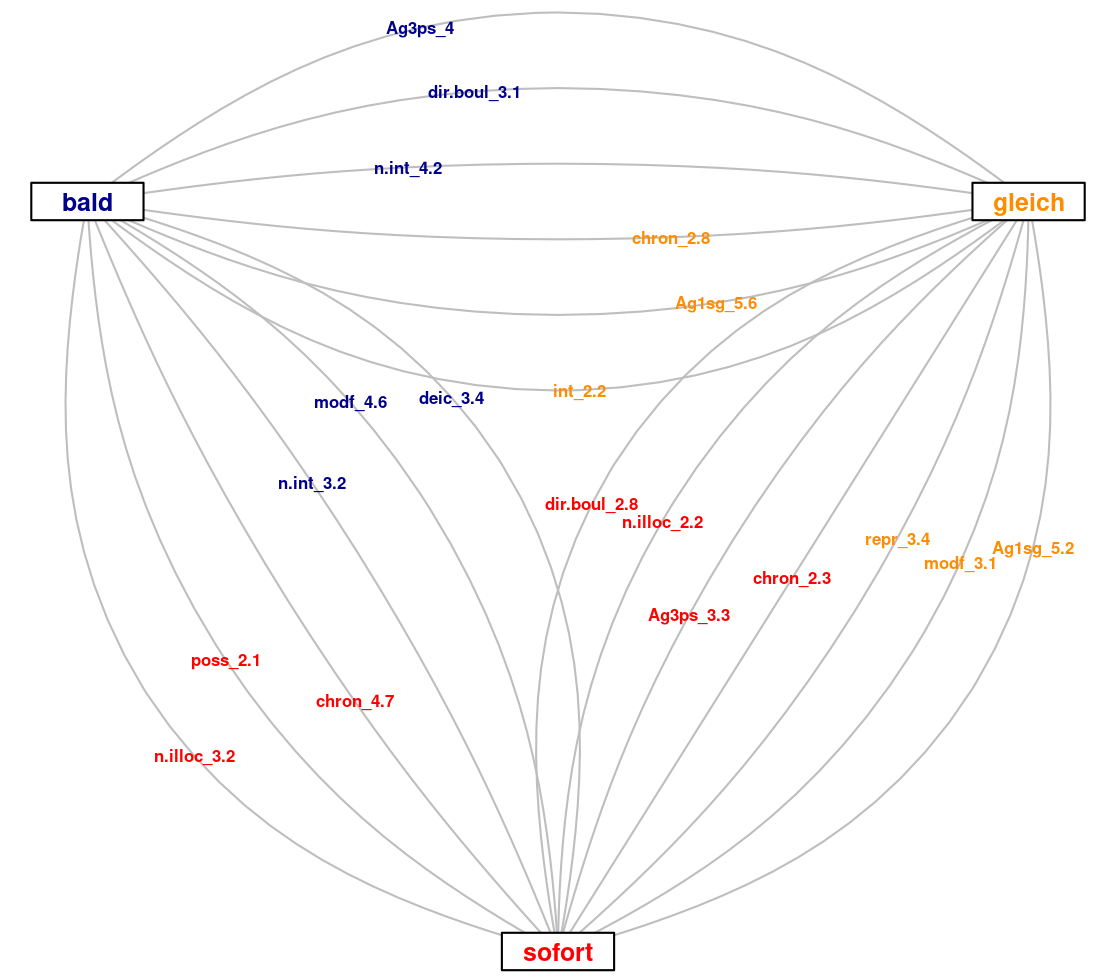
\includegraphics[width=\linewidth]{figures/CCCG-de-ip.png}
  \cprotect\caption{Context-Conditional Correlation Graph; the graph
    visualizes the distribution of German \pradv s relative to four
    variables (\textsc{Intentionality}, \textsc{Agent}, \textsc{Reference point} and
    \textsc{Illocutionary force}; see Note \ref{FigNote1} for the levels). It
    was created with the package \verb+qgraph+ for R
    \citep{qgraph-package}; cf. the script \verb+02_CCCG.R+ in the
    Supplementary Materials.}
  \label{fig:CCCG}
\end{figure}
%
The graph in Figure \ref{fig:CCCG} only shows pairwise associations
and, in a way, summarizes the information distributed over a large
number of $2\times 2$ cross-tables. In order to understand the interplay and
mutual dependencies between the variables in a multivariate data set
like ours, it often makes sense to use ordination techniques, to which
we turn now.

\subsection{Ordination}\label{sec:Ordination}

%The term `ordination' subsumes a number of methods that make use of
%`latent space', i.e., space constituted by latent variables --
%variables that are not directly observable but can be inferred from
%observable (`manifest') variables.
%%
%In the social sciences researchers often
%work with variables that are not measurable but reflected in attitudes
%or behaviour. For example, `sense of belonging' cannot be measured
%directly, but it can be inferred from responses to stimuli such as
%``Spain is my nation'' and ``I feel Spanish''
%\citep{BollenMedrano1998,Bollen2002}.

The term `ordination' subsumes a number of methods that represent multivariate data 
in a low-dimensional space. 
%The resulting dimensions are often interpreted as a `latent space', i.e., a space constituted by latent variables -- variables that are not directly observable but can be inferred from observable (`manifest') variables.
%
%In the social sciences, researchers often work with variables that are not directly measurable but are reflected in attitudes or behaviour.
%For example, a `sense of belonging' cannot be measured directly, but it can be inferred from responses to stimuli such as ``Spain is my nation'' and ``I feel Spanish'' \citep{BollenMedrano1998,Bollen2002}.
%
In this section we discuss two types of ordination techniques that are
useful for the analysis of categorical data, i.e., (simple symmetric)
Correspondence Analysis (Sects. \ref{sec:CA}) and Multiple Correspondence
Analysis (Sect. \ref{sec:MCA}).

\subsubsection{Simple symmetric Correspondence Analysis}\label{sec:CA}

Correspondence Analysis (CA) is probably the most basic type of
ordination (see \citealt{Greenacre2016} for a comprehensive overview
of the ordination techniques discussed in this section). It is based
on the idea that contingency tables can be interpreted as coordinate
systems. Consider the left-hand side of Table \ref{tab:PropTable}. The
table shows rowwise relative frequencies of the German adverbials
\textit{gleich}, \textit{sofort} and \textit{unverzüglich} as
translations of the French \ipadv s \textit{immédiatement} or
\textit{tout de suite} (so essentially it shows the distribution of
German \ipadv s in translations from French).  Each row corresponds to
a `row profile', with the percentages adding up to 1. The columns
represent three levels of the variable \textsc{Illocutionary
  force/modality}, i.e., `comm[issive]' (promises),
`dir[ective]/boul[etic]' (utterances with directive illocutionary
force or bouletic modality, where the speaker expresses a desire,
often amounting to an indirect directive), and `repr[esentative]'
(descriptions of the world).

Without providing any information about significant deviations from
the independence model the row profiles illustrate associations
between levels. For example, the table suggests that \textit{gleich}
is associated with representative illocutionary force, as 72\% of its
cases occur with that level, while for the other adverbials this
column only shows 53\% (\textit{sofort}) and 22\%
(\textit{unverzüglich}).


\begin{table}[b]
  \centering
  \begin{tabular}[h]{l|lll|lll}
    & \multicolumn{3}{l|}{row profiles} & \multicolumn{3}{l}{standardized residuals}\\ \cline{2-7}
    & comm  & dir/boul      &  repr & comm  & dir/boul      &  repr \\\hline
    \textit{gleich}       & 0.16  & 0.12          & 0.72 & 0.11  & -0.23  & 0.13\\
    \textit{sofort}       & 0.06  & 0.41          & 0.53 & -0.1 &  0.09  & -0.03\\
    \textit{unverzüglich} & 0.11  & 0.67          & 0.22 & 0.01  & 0.21   & -0.17 \\\hline
  \end{tabular}
  \caption{Table with row profiles (left) and standardized residuals
    (right) for German \ipadv s in translations from French, relative
    to the variable \textsc{Illocutionary force}}
  \label{tab:PropTable}
\end{table}

We can regard the columns of the left-hand side of Table
\ref{tab:PropTable} as constituting a coordinate system within which
we can locate the three adverbials of interest. This is illustrated in
Figure \ref{fig:Ordination1}. The three axes originating at
$(0\; 0\; 0)$ (the origin) represent the three columns of the left-hand side
of Table \ref{tab:PropTable} and constitute a three-dimensional
coordinate system. The adverbial \textit{unverzüglich}, for instance, is located
at the coordinate $(0.11\; 0.67\; 0.22)$, corresponding to the third
row profile in Table \ref{tab:PropTable} (cf. the orthogonal lines
emanating from the relevant point). The plot also shows the centroid
of the three row points (see Sect. \ref{sec:AppOrdination} in the
Appendix on how the centroid is calculated).

\begin{figure}[t]
  \centering
  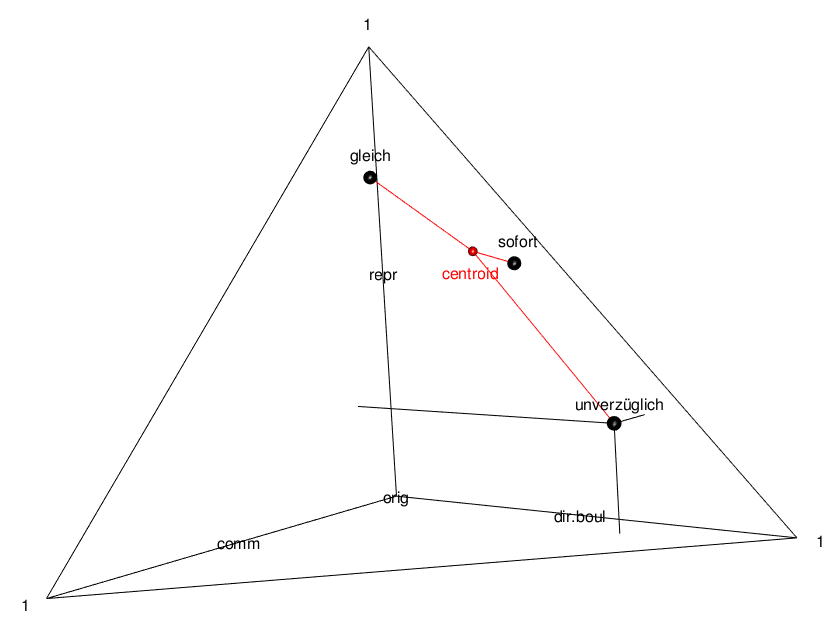
\includegraphics[width=0.75\linewidth]{figures/coord-system-1.png}
  \cprotect\caption{Visualizing Table \ref{tab:PropTable}, with the columns
    constituting a coordinate system for the rows. The plot was
    generated with the package \verb+rgl+ for \verb+R+
    (\citealt{rgl-package}).}
  \label{fig:Ordination1}
\end{figure}

The type of visualization shown in Figure \ref{fig:Ordination1}
constitutes the basis for a lower-dimensional visualization using
CA, which fits a new coordinate system to
the data, in such a way that the largest amount of `inertia'
is captured on a low number of (so-called `principal') axes --
ideally two, as two axes can be easily visualized.
%
Inertia is a measure of spread for count data around the independence
model, corresponding to variance, which is a measure of spread around
the mean value for continuous data.
%
Inertia thus measures the degree to which a contingency table deviates from
statistical independence.
%
The term is inspired by the `moment of inertia' in mechanics, which
quantifies the distribution of mass around an axis of rotation.

CA proceeds as follows:
%
first, the original contingency table (see Table \ref{tab:contingency}
on p. \pageref{tab:contingency}) is converted into a percentage table,
and then into a table of standardized residuals through division by
the square root of the expected percentage (see the right-hand side of
Table \ref{tab:PropTable}; cf. also Sect. \ref{sec:SVD}).
%
As mentioned in Sect. \ref{sec:PropGeom}, Pearson residuals
indicate deviation from independence. The resulting matrix thus
indicates to what extent a cell deviates from the independence model
(assuming a homogeneous distribution).
%
The centroid of the rows constituting this matrix is the origin of a
three-dimensional coordinate system, which is rescaled along the three
axes as a result of the standardization (division by the square root
of the expected frequency). 
The standardized residuals from Table \ref{tab:PropTable} are
visualized in Figure \ref{fig:Ordination3}.

\begin{figure}[t]
  \centering
  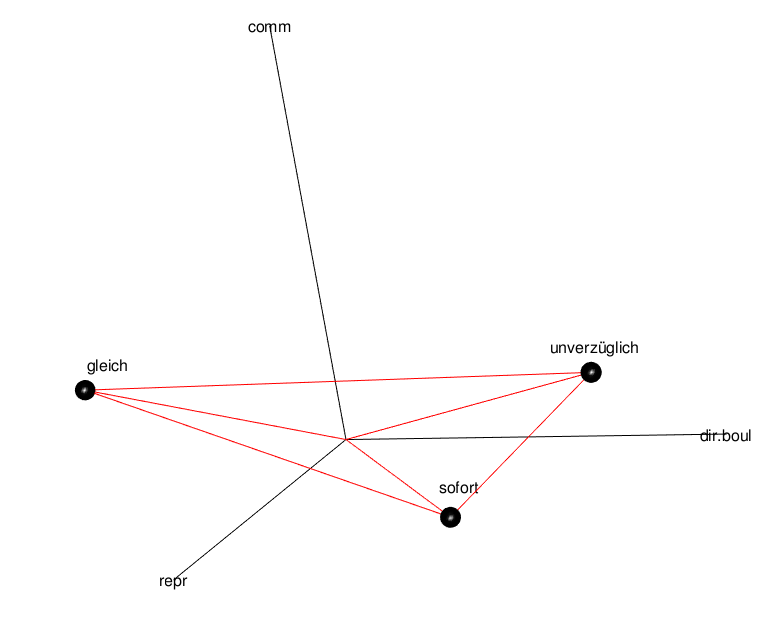
\includegraphics[width=0.75\linewidth]{figures/Ordination3b.png}
  \cprotect\caption{Visualizing the standardized residuals as shown on
    the right-hand side of Table \ref{tab:PropTable}.  The plot was
    generated with the package \verb+rgl+ for \verb+R+
    (\citealt{rgl-package}).}
  \label{fig:Ordination3}
\end{figure}

In a second step, the matrix of standardized residuals is subject to
an operation called `singular value decomposition' (SVD).  The
mathematical procedure of SVD is outlined in
Sect. \ref{sec:AppOrdination} in the Appendix (based on
\citealt{Greenacre2016}). In the main text we will focus on the
results.

SVD fits a new coordinate system to the data, in such a way that the first
(`principal') axis captures most of the inertia, the second axis,
which is orthogonal to the first, captures most of the remaining
inertia, and so on until all data points can be precisely located in
the newly created system.
%
In the case of the data visualized in Figure \ref{fig:Ordination3}, we
can find a coordinate system with only two dimensions that preserves
all the information contained in the table of standardized residuals,
because three points are always located on a (two-dimensional) plane.
If a table has been centered, as in the case
of Pearson residuals, this plane moreover contains the origin
(cf. the triangle in Figure \ref{fig:Ordination3}).

The principal axes determined with SVD %Singular Value Decomposition
constitute the axes of a new coordinate system in which we can locate
both the data points corresponding to the rows of the table of
standardized residuals -- in our case, the \ipadv s \textit{gleich},
\textit{sofort} and \textit{unverzüglich} -- and the original axes
corresponding to the levels of the variable \textsc{Illocutionary
  Force} (`comm', `dir.boul', `repr'). A CA created with the package
\verb+ca+ for \verb+R+ \citep{ca-package} is visualized in Figure
\ref{fig:Ordination2}.\footnote{In Python, the module \verb+prince+
  can be used for CA.}

\begin{figure}[t]
  \centering
  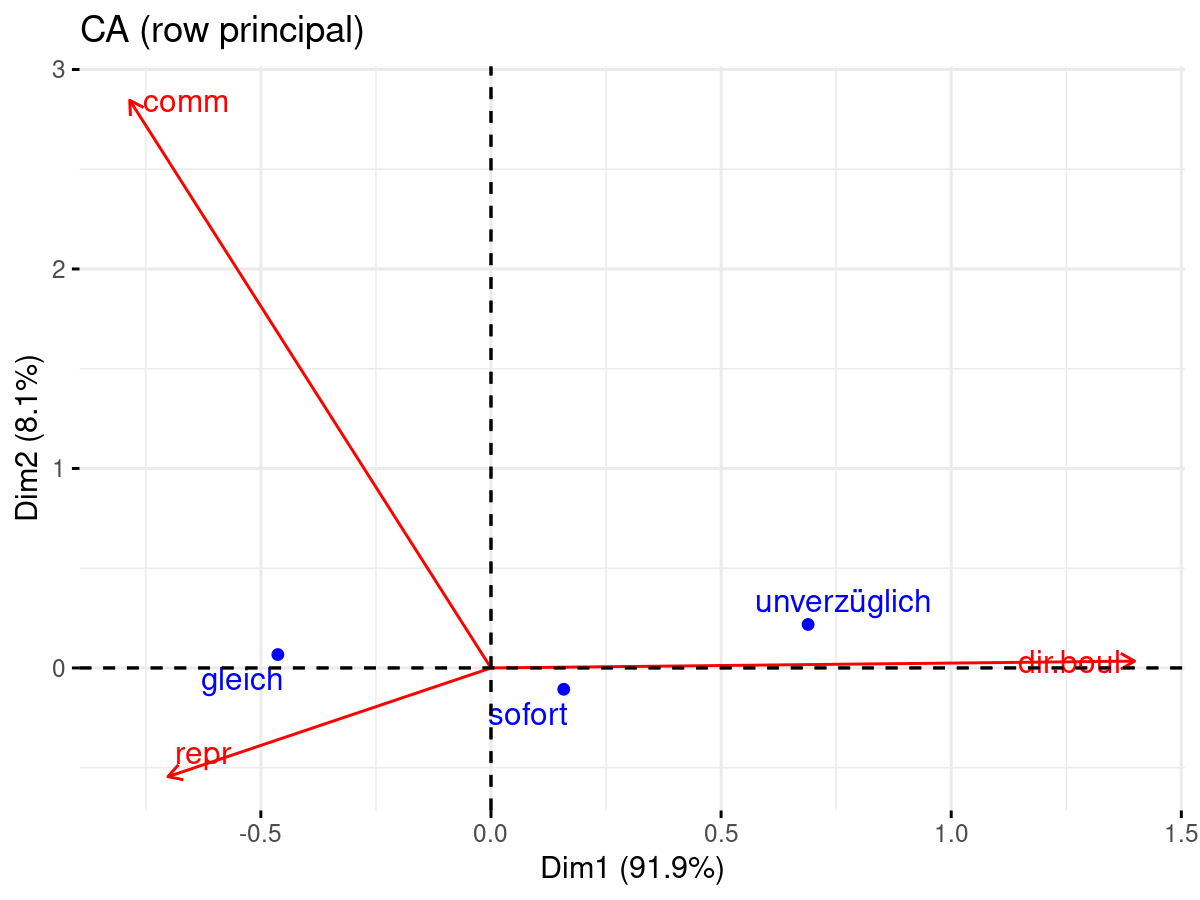
\includegraphics[width=0.75\linewidth]{figures/CA-de-illoc.png}
  \cprotect\caption{Correspondence Analysis for the data in Table
    \ref{tab:PropTable}. The CA was created with the package
    \verb+ca+ for \verb+R+ \citep{ca-package}. For the
    visualization we used the package \verb+factoextra+
    \citep{factoextra-package}. The plot shows a `row analysis', with
    row points in principal coordinates and column vectors in standard
    coordinates.}
  \label{fig:Ordination2}
\end{figure}
%

Along with the two-dimensional representation of the standardized
residuals Figure \ref{fig:Ordination2} shows percentages on both
axes. These percentages indicate how much inertia the
relevant axis covers.
%
Inertia has a direct connection to the Chi-squared test: it is
identical to the Chi-squared statistic, divided by the number of
observations; it is also the square root of the $\phi$-coefficient, a
correlation measure for contingency tables; and it relates directly to
the Chi-squared distances of the row coordinates to the origin. The
Chi-squared distance is defined as the square root of the sum of the
squared differences between the observed values and the expected
values, divided by the expected values. It is a measure of deviation
from independence. 
The inertia of the table is the sum of the Chi-squared distances squared, and
weighted by the row masses.

Consider Figure \ref{fig:Inertia} for
illustration. The left-hand side shows the squared distances of the
three coordinates representing the \ipadv s to the origin,
corresponding to the inertia (without scaling by the row masses). The
right plot shows squares based on the lines that run parallel to the
x-axis (the first principal axis) from the three \ipadv s (also unweighted
by the row masses). The area covered by the squares in the right plot
amounts to $91.9\%$ of the area covered by the total inertia as shown
in the left plot. This is what the percentage on the x-axis in Figure
\ref{fig:Ordination2} indicates.

\begin{figure}[t]
  \centering
  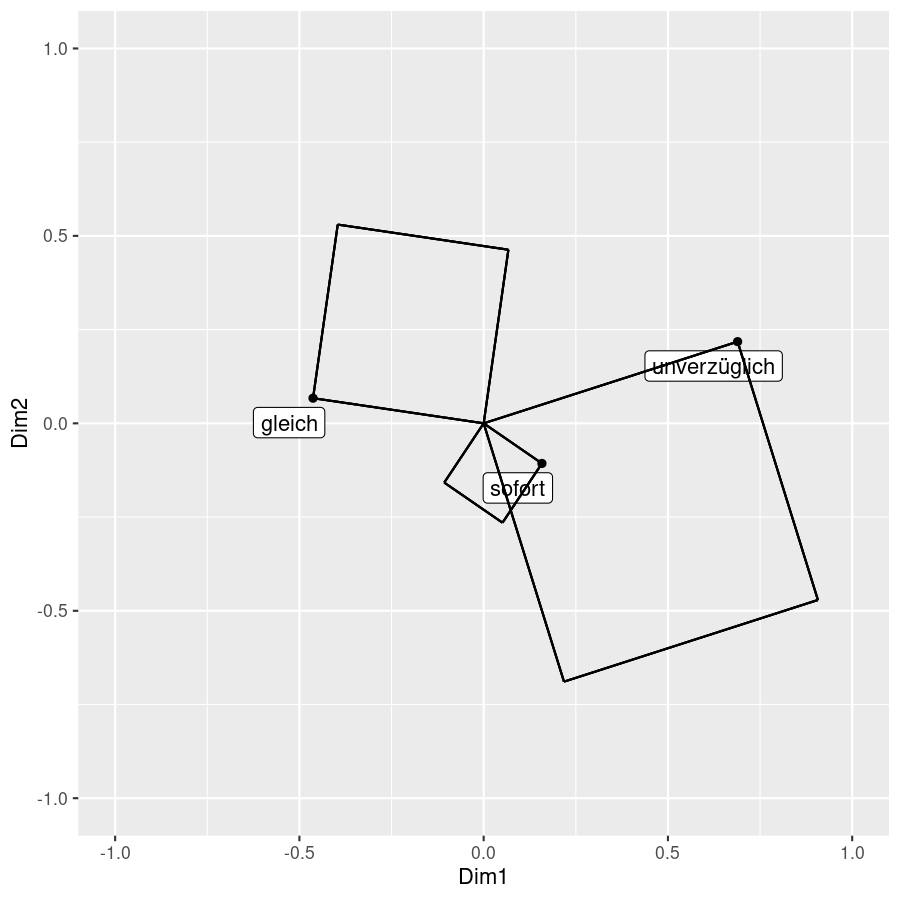
\includegraphics[width=0.45\linewidth]{figures/skewed-rects.png}
  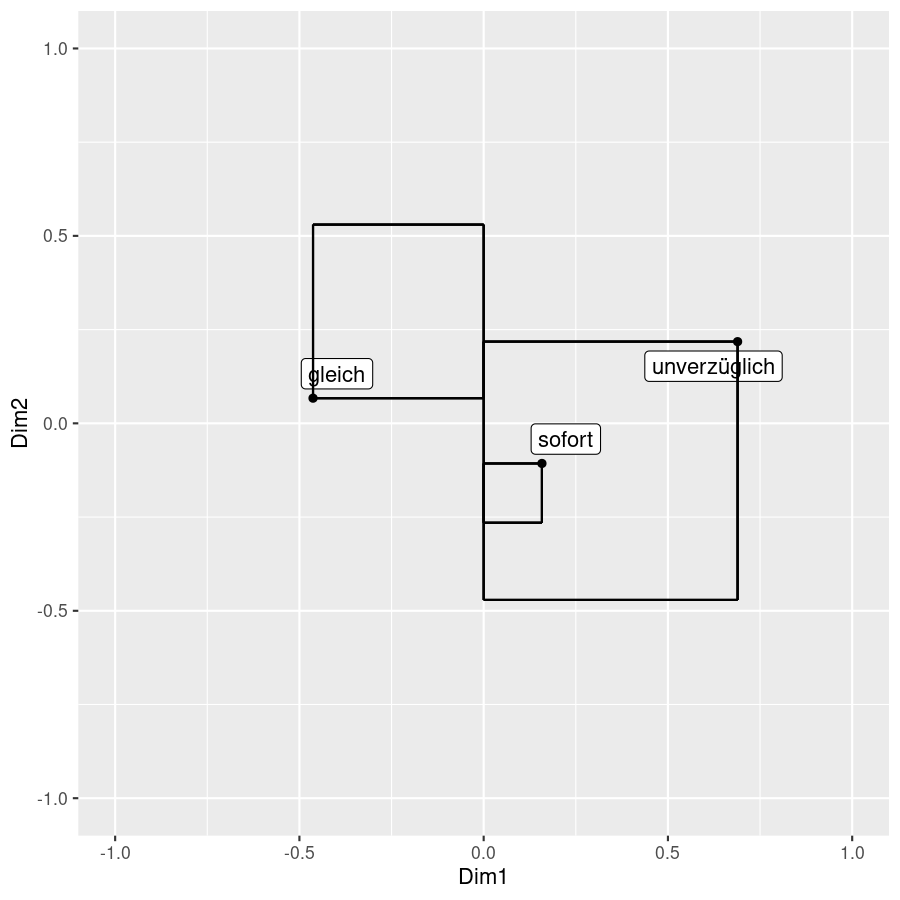
\includegraphics[width=0.45\linewidth]{figures/straight-rects.png}
  \cprotect\caption{Squared Chi-squared distances (left) and squared
    Dimension 1 coordinates (right). The plot was generated with the
    packages \verb+ggplot2+ and \verb+ggrepel+ for \verb+R+
    \citep{ggplot2-package,ggrepel-package}.}
  \label{fig:Inertia}
\end{figure}

The inertia not only gives us information about the
degree of truthfulness of the dimensionality-reduced representation
relative to the original, higher-di\-mension\-al one, it also tells us how
`important' specific axes are. When looking at Figure
\ref{fig:Ordination2} one might be led to believe that the two axes
explain a similar amount of inertia; but Axis 1 alone explains $\approx 92\%$ of
it. 
Note that all adverbials as well as the two
levels of \textsc{Illocutionary force} (`repr', `dir/boul') are very close to
the $x$-axis -- with low values on the $y$-axis --, implying that the
$y$-axis explains a low amount of their row inertia.

So far we have focused on the position of the points representing the
rows (\ipadv s) in what is called a ``row analysis'' of CA. Remember
that our starting point was the location of \ipadv s relative to distributional
variables, which constitute a coordinate system within which we can locate the
latter. In principle, CA is symmetrical and we could just as well
locate columns relative to rows. In fact, there are many ways of
visualizing CAs, implemented, for instance, in the
\verb+fviz_ca_biplot+ function of the \verb+factoextra+ package
\citep{factoextra-package}, or the \verb+plot.ca+ function of the
\verb+ca+ package for \verb+R+ \citep{ca-package}.  In a row analysis
the rows (\ipadv s) are represented in so-called `principal
coordinates', which preserve Chi-squared distances between the
observations. The columns, represented as vectors in Figure
\ref{fig:Ordination2}, are displayed in `standard coordinates', which are
so-called because they have a mean value of 0 and a variance of 1
\citep[62]{Greenacre2016}.

\hyphenation{gleich}

In this display the relationship between an \ipadv\ (row) and a
variable (column) is not represented by the distances between row and
column vectors; it (ideally) corresponds to the inner products of
these vectors (``ideally'' bacause information may be lost as a result
of the dimensionality reduction). This means that the degree of
association between a row and a column is a function of the degree to
which the two vectors point in the same direction. If all of the
information has been preserved, we can reconstruct the values
of the original table from the map shown in Figure
\ref{fig:Ordination2}. For example, the standardized residual for the
combination \textit{gleich}/`repr' is the inner product of the two
vectors for \textit{gleich} (scaled by the square root of its row
mass) and the vector pointing at `repr' (scaled by the square root of
the average profile; see \citealt{Greenacre2016} for more information
and Sect. \ref{sec:AppOrdination} in the Appendix for the calculation of this
example).

While not everybody may be interested in the mathematical details, it
is important to be aware of the specific type of map that is used for
visualization. The `row principal' representation chosen in Figure
\ref{fig:Ordination2} is rather transparent, but often has the
disadvantage of a visual imbalance between the row points, which are
closer to the centre, and the column points, which are spread out
more. Users should be aware, however, that a representation that
condenses the data -- while visually being more pleasing --
potentially does not have the inner product interpretation of an
asymmetric row principal plot, where the rows are represented in
principal coordinates, and the columns in standard coordinates (see
\citealt[Ch. 13]{Greenacre2016} for discussion).

Representations like the one in Figure \ref{fig:Ordination2} give us
an idea of the relationship between the levels of two
variables. However, with a multivariate data set like ours, we need to
be able to represent relationships between more than one variable. A
very simple way of visualizing more than one variable is provided by a
`stacked' CA \citep[Ch. 17]{Greenacre2016}. We can simply concatenate
contingency tables (horizontally or vertically) and carry out a CA on
that table. Horizontal concatenation is illustrated for our data in
Table \ref{tab:StackedContingency}, which shows the percentages for
the variable \textsc{Illocutionary force} on the left, and for
\textsc{Agent} on the right.

\begin{table}[t]
  \centering
  \begin{tabular}[h]{l|lll|llll}
             &  comm  &  dir.boul &  repr &  1pl  &  1sg  &  2ps  &  3ps\\\hline
\textit{gleich}       &  0.08  &  0.06     &  0.36 &  0.06 &  0.22 &  0.06 &  0.16\\
\textit{sofort}       &  0.03  &  0.21     &  0.26 &  0.07 &  0.01 &  0.06 &  0.35\\
\textit{unverzüglich} &  0.06  &  0.33     &  0.11 &  0.06 &  0.00 &  0.00 & 0.44\\
  \end{tabular}
  \caption{Stacked contingency table for German \ipadv s (in
    translations from French) and the explanatory variables
    \textsc{Illocutionary force} and \textsc{Agent}}
  \label{tab:StackedContingency}
\end{table}
%
Given that the number of observations per variable is invariant, the
Chi-squared distances between the levels of each variable are preserved
in this type of stacked CA. The positions of the various levels
relative to each other are thus not affected by the stacking
(cf. Figure \ref{fig:Ordination5}). However, it is clear that some
information is lost in a stacked CA, as we do not get any information
about the relationship between the levels of the explanatory variables
(here, \textsc{Illocutionary force} and \textsc{Agent}). Table
\ref{tab:StackedContingency} suggests that a certain number of
ocurrences of \textit{gleich} have commissive illocutionary force, and
another set of observations has a first person agent. The table does
not tell us how many of the commissive observations have first person
agents. In other words, the distributional variables are treated as
being independent. While this is a clear drawback of the stacked CA,
the method can be useful in order to determine the degree of
independence of predictor variables. In particular, it can be
instructive to compare a stacked CA to a Multiple Correspondence
Analysis, to which we turn next.

\begin{figure}[b]
  \centering
  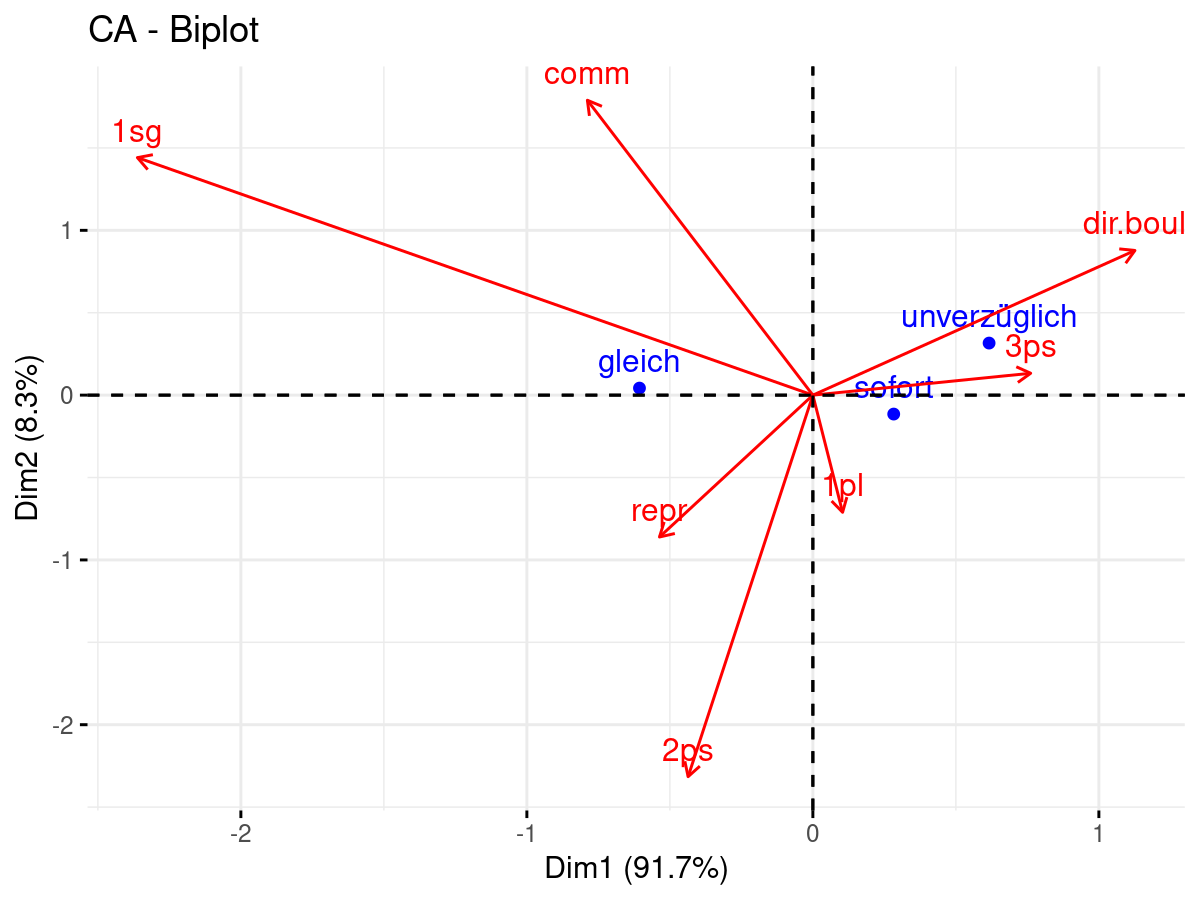
\includegraphics[width=0.67\linewidth]{figures/CA-de-stacked.png}
  \cprotect\caption{Stacked Correspondence Analysis showing the
    location of three German \pradv s in a coordinate system derived from their associations with
    the variables \textsc{Illocutionary force} and \textsc{Agent}. The
    CA was fitted with the package \verb+ca+ for \verb+R+
    (\citealt{ca-package}) and the plot was created with the package
    \verb+factoextra+ for \verb+R+ \citep{factoextra-package}.}
  \label{fig:Ordination5}
\end{figure}

\subsubsection{Multiple Correspondence Analysis}\label{sec:MCA}

From a mathematical point of view, Multiple Correspondence Analysis
(MCA) functions very much like (simple) CA. However, it is based on a
representation of the data that takes the relationships between all
(explanatory as well as response) variables into account. There are
two (near equivalent) ways of accomplishing this: (i) carrying out a CA on
the indicator matrix of a data set, or (ii) using the Burt table
instead.

An indicator matrix is a binary matrix that indicates whether
or not an observation exhibits a given property.
%
Consider Table \ref{tab:RandomDF}, which shows a random fragment of
our data frame (German translations of French \ipadv s). Each row corresponds to
one example, and the columns specify the illocutionary force, the Agent, and
the German adverbial.

\begin{table}[H]
  % \centering
  \small
  \begin{tabular}[h]{llll}
  ID  &    \textsc{Illoc}    & \textsc{Agent}    & German \textsc{\ipadv}\\\hline
  214 &   repr      &    1sg   &    \textit{sofort}\\
  216 &   dir.boul  &    1pl   &    \textit{sofort}\\
  217 &   repr      &    3ps   &    \textit{gleich}\\
  218 &   repr      &    3ps   &    \textit{sofort}\\
  221 &   dir.boul  &    3ps   &    \textit{unverzüglich}\\
  \end{tabular}
  \caption{Random fragment of the data frame}
  \label{tab:RandomDF}
\end{table}
%
The indicator matrix corresponding to Table \ref{tab:RandomDF} is
shown in Table \ref{tab:RandomDFIndicator}.
%
Here, each column corresponds to a level of a variable, not a variable. While
Table \ref{tab:RandomDF} specifies the levels themselves in the cells,
Table \ref{tab:RandomDFIndicator} shows whether (1) or not (0) the observation
in question is an instance of the relevant level.

\begin{table}[H]
  % \centering
  \small
  \begin{tabular}[h]{l|rrr|rrrr|rrr}
    & \multicolumn{3}{c|}{\textsc{Illoc}} & \multicolumn{4}{c|}{\textsc{Agent}} & \multicolumn{3}{c}{\textsc{\ipadv}}\\ 
    &   comm & dir.boul & repr & 1pl & 1sg & 2ps & 3ps & \textit{gleich}& \textit{sofort} & \textit{unvzgl.}\\\hline
214 &     0  & 0        &  1    &   0 & 1           & 0           & 0           & 0           & 1       & 0\\
215 &     0  & 1        &  0    &   1 & 0           & 0           & 0           & 0           & 1       & 0\\
216 &     0  & 0        &  1    &   0 & 0           & 0           & 1           & 1           & 0       & 0\\
217 &     0  & 0        &  1    &   0 & 0           & 0           & 1           & 0           & 1       & 0\\
218 &     0  & 1        &  0    &   0 & 0           & 0           & 1           & 0           & 0       & 1\\    
  \end{tabular}
  \caption{Indicator matrix corresponding to Table \ref{tab:RandomDF}}
  \label{tab:RandomDFIndicator}
\end{table}

A Burt matrix is a cross-tabulation of the frequencies of all levels of
all variables with all other levels of all other variables. Table
\ref{tab:BurtMat} shows a fragment of our data in the form of a Burt
matrix. Burt matrices and indicator matrices are systematically
related insofar as the Burt matrix is the inner product of the
transpose of the indicator matrix with itself ($B=I^\mathsf{T}I$, for
an indicator matrix $I$).

While MCA is ``mathematically'' quite similar to CA, 
from the point of view of interpretation the two techniques are quite
different. In CA, the rows correspond to categories of interest and the
columns to the levels of a variable. In MCA, the rows correspond to
individual observations (in the indicator matrix) and the columns
correspond to variables that the individuals do (not) exhibit. Unlike
CA, MCA thus provides information about individual
observations. Moreover, in MCA \textit{all} (levels of) variables are
related to each other via Chi-squared distances.


\begin{table}[t]
  \centering
  \begin{tabular}[h]{l|lll|lll}
               & \textit{gleich} & \textit{sofort} & \textit{unverzüglich} & comm & dir.boul &repr\\\hline
\textit{gleich}         & 25            & 0                  & 0                & 4 & 3               & 18\\
\textit{sofort}         & 0           & 34                  & 0                & 2 & 14               & 18\\
\textit{unverzüglich}   & 0            & 0                  & 9                & 1 & 6                & 2\\\hline
comm           & 4            & 2                  & 1                & 7 & 0                & 0\\
dir.boul       & 3           & 14                  & 6                & 0 & 23                & 0\\
repr           & 18           & 18                  & 2                & 0 & 0               & 38\\
  \end{tabular}
  \caption{Burt matrix corresponding to Table \ref{tab:RandomDF}}
  \label{tab:BurtMat}
\end{table}

A downside of MCA is that the underlying data tables -- the indicator
matrix (Table \ref{tab:RandomDFIndicator}) or the Burt matrix (Table
\ref{tab:BurtMat}) -- are highly redundant. The indicator matrix
contains a lot of zeros, which turn into negative values when the
residuals are calculated. The Burt matrix contains a lot of
uninformative material on the diagonal, where levels are crossed with
themselves. Because of the redundancy, both tables inflate the overall
inertia. As a result, MCAs typically appear to explain a low
percentage of inertia on their first principal axes.
%
\citet{Greenacre2016} has proposed a way of `adjusting' the inertia in
MCAs, which is implemented in the package \verb+ca+ for
\verb+R+ \citep{ca-package}. 

Figure \ref{fig:Ordination6} shows an MCA for German translations of
French \ipadv s, with three variables: \textsc{\ipadv},
\textsc{Illocutionary force} and \textsc{Agent}.\footnote{We used the
  package \verb+FactoMineR+ for \verb+R+
  \citep{FactoMineR-package}. In Python, the module \verb+prince+ can
  be used for MCAs.} Without adjustment, the percentage of inertia
captured by the first two principal axes is 26.3\% (Axis 1) and 19.2\%
(Axis 2). It is much higher when computed with Greenacre's (2016)
adjustment (72.7\% [Axis 1] and 11.0\% [Axis 2]).

\begin{figure}[t]
  \centering
  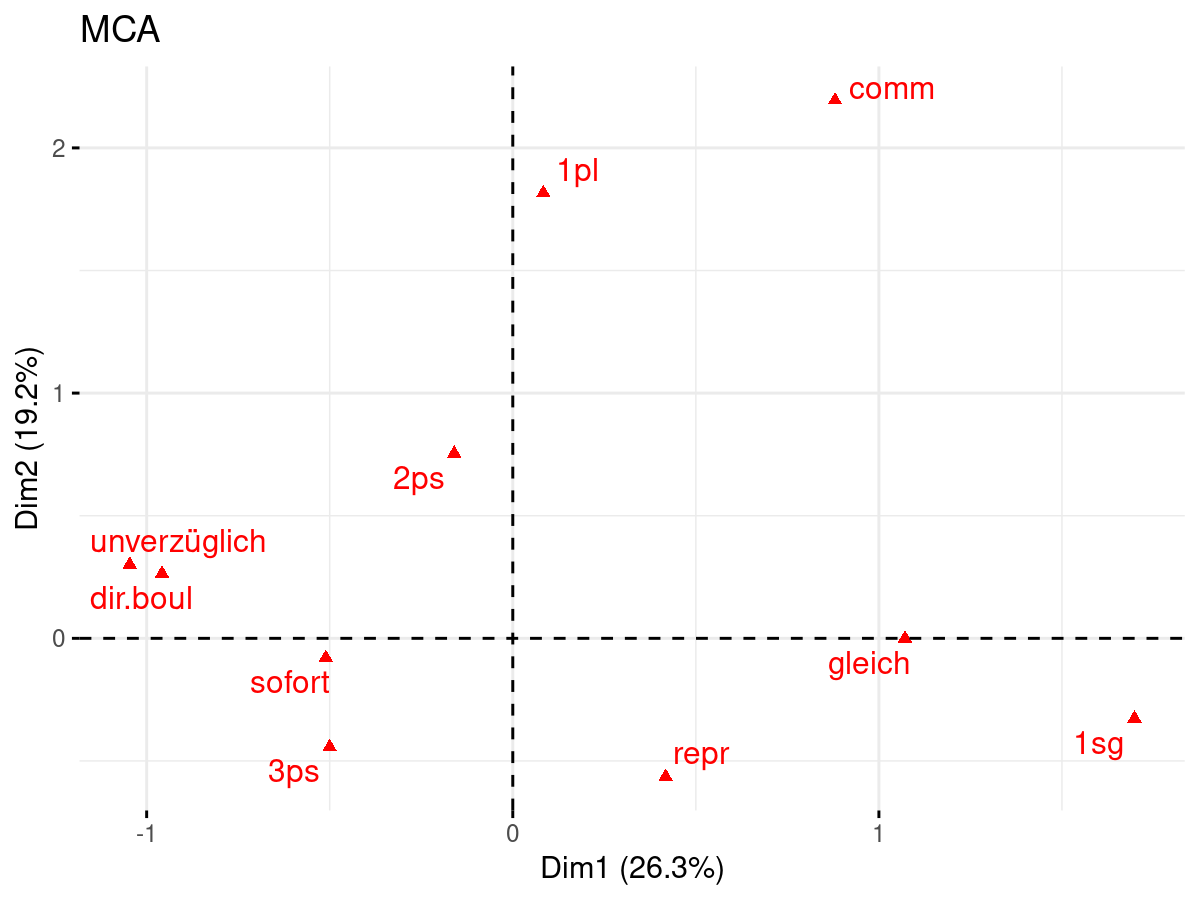
\includegraphics[width=0.75\linewidth]{figures/MCA-de-trl.png}
  \cprotect\caption{Multiple Correspondence Analysis for the variables
    \textsc{Illocutionary force}, \textsc{Agent} and \textsc{\ipadv}
    (German translations of French \ipadv s). The MCA was fitted with
    the package \verb+FactoMineR+ for \verb+R+
    \citep{FactoMineR-package}, the plot was generated using the
    package \verb+factoextra+ \citep{factoextra-package}.}
  \label{fig:Ordination6}
\end{figure}

An MCA creates a new coordinate system that is structured by all variables
relative to all other variables. It creates a mapping from frequency
distributions to positions in this system. We can therefore also locate
variables (and observations) in MCA-coordinates without them being used
to create those coordinates. In MCA speech, this means that we use
`supplementary' (or `passive') variables. In a data set like ours it
often makes sense to treat the target variable -- in our case,
expressions of immediate or proximal posteriority -- as a
supplementary variable. The idea is that the MCA-coordinates are
defined by explanatory variables only, and that the adverbials in
question can be located in terms of these coordinates. This is shown in
Figure \ref{fig:Ordination7} for the same data that was used to
generate the stacked CA in Figure \ref{fig:Ordination5}, and the MCA
without supplementary variables in Figure \ref{fig:Ordination6}.


\begin{figure}[t]
  \centering
  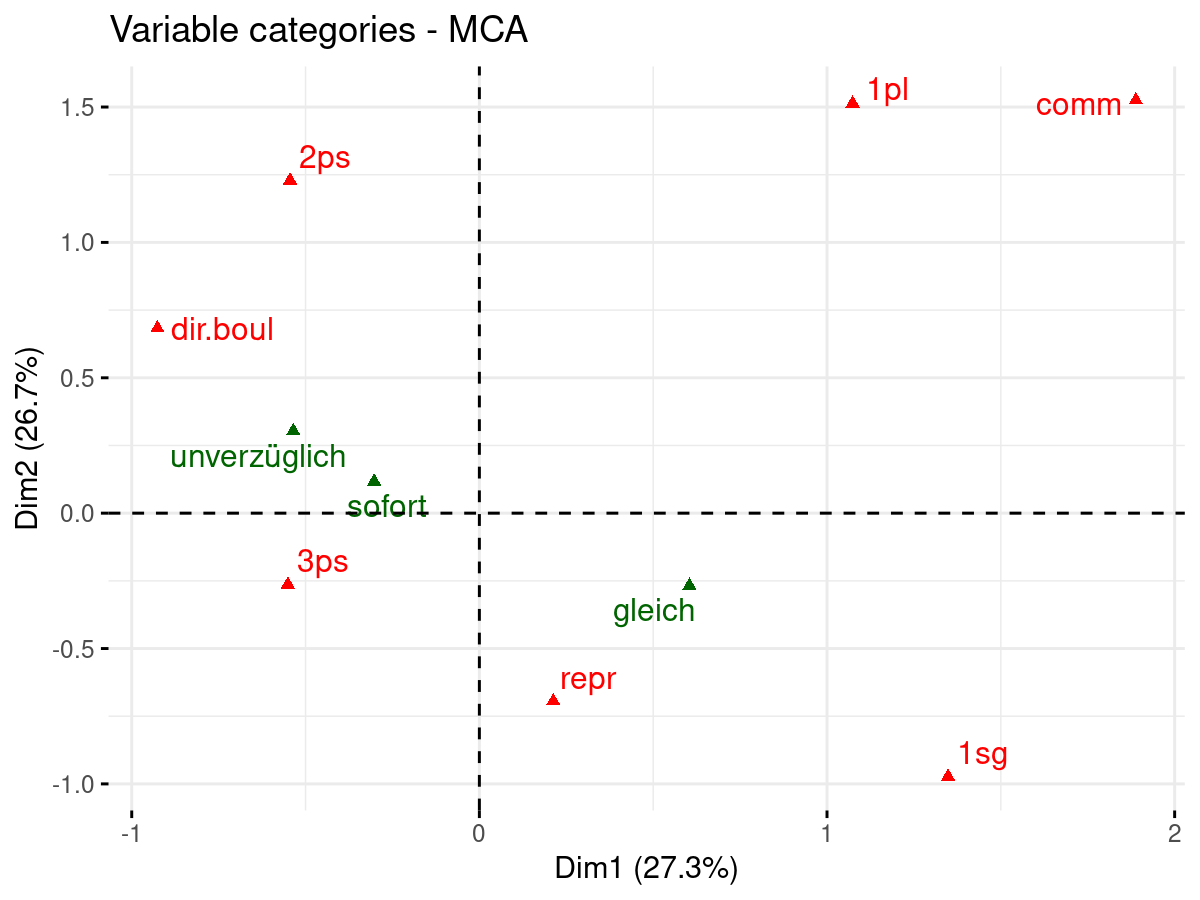
\includegraphics[width=0.75\linewidth]{figures/MCA-supp-de-trl.png}
  \cprotect\caption{MCA for the variables \textsc{Illocutionary force}
    and \textsc{Agent}, with \textsc{\ipadv} as a supplementary
    variable (German translations of French \ipadv s).)  The MCA was
    fitted with the package \verb+FactoMineR+ for \verb+R+
    \citep{FactoMineR-package}, the plot was generated using the package
    \verb+factoextra+ \citep{factoextra-package}.}
  \label{fig:Ordination7}
\end{figure}

\subsection{Comparing CA and MCA}\label{sec:OrdionationComparison} 

The three ordination methods mentioned above provide ways of
displaying different types of interdependencies between variables. A
stacked CA represents the data in a coordinate system derived from the
association between rows and columns, and positions the rows
(adverbials) relative to the columns (distributional variables), or
vice versa (the method is symmetric, although our focus has been on the
row analysis). CA visualizes relations between context variables
and adverbials, but not relations among the context variables
themselves.

An MCA with supplementary variables, in a sense, emphasizes the
opposite perspective: it constructs a space based on the relationships
among the context variables, and then projects the adverbials into this
space. An MCA without supplementary variables represents relationships
among all variables simultaneously, i.e., it does not distinguish
between context variables and adverbials.


The differences between the three types of visualizations can be
illustrated with the relationship between one German adverbial,
\textit{unverzüglich}, and two context variables,
\textsc{Illocutionary force} and \textsc{Agent}. Consider first the
(stacked) CA shown in Figure \ref{fig:Ordination5}. The \ipadv\
\textit{unverzüglich} and the category `2nd person' are located on opposite
ends of the origin, suggesting a negative association. As a matter of
fact, the variables are complementary, in the sense that
\textit{unverzüglich} is never used with the second person in our
sample. In Figures \ref{fig:Ordination6} (MCA without supplementary
variables) and \ref{fig:Ordination7} (MCA with supplementary
variables), the second person is located in the same quadrant as
\textit{unverzüglich}. The reason is that both categories are
distributionally related to directive illocutionary force or bouletic
modality (`dir.boul'), though not to each other. In a way, the MCAs
suggests a deceiving distributional association between
\textit{unverzüglich} and the second person.
%
What this example illustrates is that none of the three methods
considered above -- stacked CA, MCA with or without supplementary
variables -- can, in itself, provide a complete picture of the
data. It is therefore instructive to experiment with different methods
in order to develop a better understanding of the data. This does not
mean, of course, that readers should feel encouraged to cherry pick
those plots that they like best. Remember that the primary focus of this
contribution is to support researchers in understanding their data,
not in applying inferential statistics.

%%% Local Variables:
%%% mode: latex
%%% TeX-master: "main"
%%% End:
